
\subsection{Definición de ABMs - Clases Admin}%
\label{sub:definición_de_abms_clases_admin}

Para definir un ABM, es decir una interfaz capaz de manejar el alta, baja y modificación de registros; es necesario una entidad. Por este motivo, para obtener
una idea general del funcionamiento de Sonata-Admin, se decidió definir algunas entidades y generar una clase admin\@.
En sonata admin, una clase admin es aquella que, dada una entidad, permite añadir un servicio en la plataforma web sonata que se hace cargo de cada una de estas funciones.

Para crear un admin es necesario extender de la clase \textbf{AbstractAdmin} que provee sonata y, mediante métodos heredados de la misma, configurar la manera en
que se muestra la información\@.
Alguno de estos métodos son:

\begin{itemize}
    \item \textit{configureFormFields:} este método define los campos a mostrarse durante la acción de crear y editar.
    \item \textit{configureListFields:} define los campos a mostrar durante la acción de listar datos.
    \item \textit{configureShowFields:} establece la información a mostrar durante la acción de Ver una entrada.
\end{itemize}

\noindent
Además de esto, una clase admin en \textbf{Sonata} permite:
\begin{itemize}
    \item Validar información
    \item Agregar acciones de acuerdo a eventos de cada entidad
    \item Establecer jerarquías entre clases admin
    \item Crear un menú de forma fácil en las vistas del admin
    \item Establecer filtros de búsqueda.
\end{itemize}

Éstas son las funcionalidades que se utilizaron en este proyecto, sonata cuenta con aún más opciones de configuración.

Una clase admin contiene una referencia a la entidad base del mismo a través de un objeto denominado Subject. Sonata utiliza este objeto para realizar
la mayoría de sus operaciones.
Para configurar las diferentes secciones del admin, es necesario especificar la información que se desea incluir, esto es posible utilizando el nombre del campo.

\begin{figure}[h]
    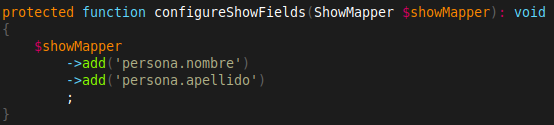
\includegraphics[width=1\linewidth]{image/show.png}
    \caption{Ejemplo de definición de campos a mostrar durante la creación/edición.\newline \textbf{Fuente:} Elaboración propia.}
    \label{fig:image/show}
\end{figure}

Si se desea acceder a asociaciones, (datos que representan la relación de una entidad) se puede hacerlo mediante una notación de puntos, por ejemplo:
Si se tiene una instancia de \textbf{Actividad}, la misma tendrá una asociación con una entidad persona. Por lo tanto se puede acceder al nombre de una persona referenciándola como ``persona.nombre''.

\subsubsection{Proyecto}%
\label{ssub:admin_proyectadmin_proyecto}

En el admin de Proyecto se agregaron los siguientes campos en cada acción:

\begin{itemize}
    \item Lista: nombre del proyecto.
    \item Ver: nombre del proyecto
    \item Inserción: nombre y roles de proyecto.
\end{itemize}

Además de esta información se agregó un menú en la barra superior de navegación de la pantalla de proyecto. El mismo permite acceder a acciones del \textit{hijo},
que en este caso sería el admin de Miembro de proyecto.

Cuando se asigna un admin como \textit{hijo}, se obtiene rutas anidadas, de forma que se puede acceder a acciones del \textit{hijo} desde la vista del padre. Ej: Una ruta
para acceder a un miembro en particular sería de la forma:\newline \textbf{/miembroproyecto/{id}/(show | edit)}\@.\newline\newline Cuando se accede a los miembros de cada proyecto se obtienen rutas de la forma:\newline \textbf{/proyecto/{id}/miembroproyecto/{id}/(show | edit)},
\newline \textbf{/proyecto/{id}/miembroproyecto/list}\newline

Para crear un proyecto, se debe proporcionar los datos de nombre y roles. Los roles de proyecto están representados en la entidad en forma de Colección,
por lo tanto se utilizó un tipo de formulario que permite la elección de opciones múltiples y además permite agregar nuevas instancias de
rol(figura~\ref{fig:image/proyecto-editar}).

\begin{figure}[h]
    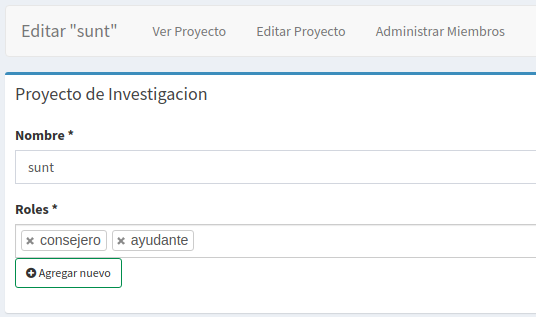
\includegraphics[width=1\linewidth]{image/proyecto-editar.png}
    \caption{Admin: Acción de  editar Proyectos.\newline \textbf{Fuente:} Elaboración propia, captura de pantalla de la aplicación web.}
    \label{fig:image/proyecto-editar}
\end{figure}

\subsubsection{Miembro de Proyecto}%
\label{ssub:miembro_de_proyecto_admin}
Para la definición del admin de miembros de proyecto se lo estableció como un \textit{hijo} de el admin Proyecto, esto es porque tiene sentido desde el punto de vista
de la relación que forman. Un proyecto estará integrado por muchos miembros, por lo tanto al asignar a miembros de proyecto como admin \textit{hijo} de Proyecto permite
administrar los miembros desde la interfaz de proyectos. Al fin y al cabo, la clase admin de miembros no tiene sentido por sí sola.

Para asignar un admin como \textit{hijo} se debe configurar el servicio padre un método denominado \textbf{addChild}. Como parámetros requiere el servicio del admin
a actuar de \textit{hijo} y el campo mediante el cual está relacionado.


Al agregar un admin como \textit{hijo} se generan las rutas anidadas (sección:~\ref{ssub:admin_proyectadmin_proyecto}), pero no se tiene una forma de acceder a
ellas desde la aplicación web\@. Una buena forma de solucionar este problema es, según la documentación de \textbf{Sonata}, agregar un menú en la barra superior
de la página que contenga botones mediante los cuales acceder a estas rutas.\textcite{sonata-childAdmin}

\begin{figure}[h]
    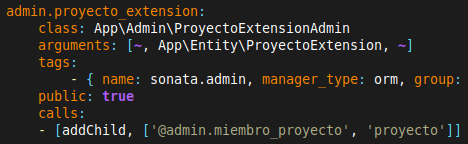
\includegraphics[width=1\linewidth]{image/addChild.png}
    \caption{Servicio admin de Proyecto de Extensión\newline \textbf{Fuente:} Elaboración propia, captura de pantalla de código fuente.}
    \label{fig:image/addChild}
\end{figure}

\newpage
\subsubsection{Rol de proyecto}%
\label{ssub:rol_de_proyecto_admin}

El admin de roles es muy básico, solo contiene el campo de nombre. Por lo tanto, en cada una de sus acciones se agregó este unico campo.


Lo interesante en este admin es que se agregó al admin de miembros como \textit{hijo}. De esta forma se puede listar los miembros que cumplen cada rol en
particular.
Esto se logra mediante el método \textbf{addChild} (figura~\ref{fig:image/addChild}) y creando un menú del mismo tipo que el definido en el admin de miembros.
